\section{Introduction}
\label{sec:introduction}









Large-scale Deep Learning (DL) training workloads, increasingly require weeks or months of compute time on GPU clusters~\cite{opt2}. As the duration and scale of these training efforts grows, so does the frequency of failures. For example, the DL training workloads in a Microsoft cluster encounter a failure every 45 minutes on average (excluding early failures) due to various system and user errors~\cite{philly}. This makes the role of checkpointing--creating periodic snapshots of a DL model during its training--increasingly crucial. When failure occurs, training can be recovered from the most recent checkpoint to reduce lost work.

During the model development phase, developers often resume from a stable mid-training checkpoint instead of starting from scratch for each bug fix or modification~\cite{opt-logbook}. Checkpoints are also used in transfer learning, where a saved model state can be adapted for\alexey{to?} a different task. Due to these varied uses, there is a growing research interest in checkpointing systems~\cite{QD, lcCompression, checknrun, deltadnn}.




Frequent checkpoints ensure minimal loss of progress in the event of failures but also increase the storage cost. For instance, checkpoints for language models like Pythia \cite{pythia}, OPT \cite{opt2} require tens of gigabytes of storage for each checkpoint. During the course of training, hundreds of such checkpoints are generated. As models grow in complexity and size, and as organizations seek to maintain a multitude of checkpoints, compressing these checkpoints becomes necessary. 



\begin{figure}
    \centering
    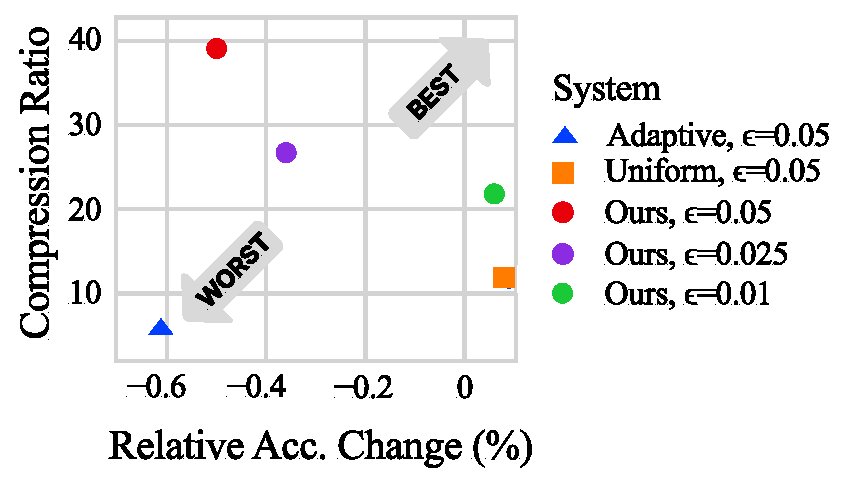
\includegraphics[width=0.9\linewidth]{figures/evaluation/fr_tradeoff_img.pdf}
    \caption{
        \small \sys provides better accuracy-storage tradeoffs compared to baselines for ResNet152 training.   }
    \label{fig:fr-tradeoff-single}
\end{figure}






As a result, several model compression systems have been proposed in the recent past \cite{QD,lcCompression,checknrun,deltadnn}, however, existing checkpoint compression systems face shortcomings in terms of suboptimal trade-off between compression ratio and accuracy degradation as shown in \cref{fig:fr-tradeoff-single}. We find that this issue originates due to the following factors. First, model parameters exhibit different levels of sensitivity to compression. Systems such as Check-N-Run \cite{checknrun} and QD-Compressor \cite{QD} adopt uniform quantization strategies that provide all parameters with the same level of resolution -- oblivious to the level of their impact on the model quality. 
Second, it's observed that models, as they accrue knowledge over the course of training, exhibit higher quantization error\alexey{either we observe or cite who observes}. However, existing systems adhere to fixed quantization configurations, e.g., a preset number of quantization bins, throughout training.




\begin{figure*}[t!]
    \centering
    \includegraphics[width=\textwidth]{figures/solution/hld_v3_img.pdf}
    \caption{
        \small High-level workflow of a checkpoint compression and saving request, and resumption of training on failure from a saved compressed checkpoint in \sys.}
    \label{fig:hld}    
\end{figure*}


To overcome these limitations, we introduce \sys---an efficient, transparent in-training model checkpoint compression system for DL workloads (\autoref{fig:hld}). \sys is premised on the observation that not all model parameters contribute equally to model quality, and this contribution varies as the model trains\alexey{varies over the course of model training}. This observation informs three main aspects of \sys.

First, \sys uses a comprehensive quantization configuration space that partitions model parameters into three groups based on their significance: parameters preserved with full precision (unchanged), pruned parameters (set to zero), and quantized parameters. For the quantized parameters, \sys proposes a novel \textit{non-uniform} quantization approach using a sketch-based approximate K-Means clustering, achieving up to 65$
\times$ speed up compared to a na\"ive implementation. This enables more effective compression by reducing the number of required quantization bins by 2-3$\times$ compared to uniform quantization. 


Second, \sys includes an efficient dynamic quantization configuration search component. This component automatically adapts the quantization configuration as parameters' sensitivity towards\alexey{to} compression changes over training time. This has the combined benefit of improving compression performance and alleviating the cognitive burden on ML practitioners to manually choose these configurations.

Finally, \sys implements a novel quantization-aware delta encoding scheme, based on the observation that most parameters remain in the same quantization bin across consecutive checkpoints.
Our delta encoding scheme rearranges the model parameters such that parameters for each quantization bucket are stored separately, improving delta encoding efficiency with compression ratios 3-4$\times$ higher than existing delta compression schemes.











\sys builds on the following key contributions:

\begin{itemize}
\item A novel \textit{non-uniform} quantization algorithm using approximate K-Means clustering. 
\item A mechanism for efficient, automatic quantization configuration search space navigation during training.
\item A delta compression algorithm with effective run length encoding enabled by quantization-aware model parameter rearrangement.


\end{itemize}

We evaluate \sys on 7 different model families, including tasks in vision and language modeling.
\sys reduces checkpoint size by 26-39$\times$ for fault-tolerant training and sustains up to ten failures (for multi-day training jobs) with negligible impact on the final accuracy of the trained model, achieving a 1.3-3.3$\times$ improvement over state-of-the-art methods. \sys can also reduce the storage overhead of snapshots of pre-trained models used for transfer learning by 10$\times$ with no impact on the performance of the fine-tuned model. Overall, \sys can achieve at least an order of magnitude checkpoint overhead reduction on both use cases with minimal accuracy loss. 
